\section{Influence Among Anti-Virus Engines}
\label{sec:influ}

Anti-virus vendors frequently use VirusTotal to identify false negatives in their products, 
which are malware they fail to detect but detected by other vendors~\cite{vt-usage}.
As discussed in Section~\ref{sec:meth}, many files are submitted to VirusTotal more than once, 
and more than 99\% submissions are analyzed by at least 50 anti-virus engines. 
Interestingly, we observe that some engines fail to identify some malware during early submissions, 
but they catch up when analyzing later submissions.

This observation led us to ask one important question that have never been studied before:
{\em is there influence across different anti-virus vendors?}
That is, can an anti-virus vendor's decision be affected by other vendors' malware detection results?
With the large number of anti-virus engines in the wild, it is important to understand if an anti-virus engine is
reliable and can be trusted.  

This section presents our answer to this question by quantifying the influence across anti-virus engines.
Specifically, we study the historical submissions of a file and
how anti-virus engines change their labels of the same file over time.
We also provide a prediction model on whether an engine will identify a file as malware in the future
after labeling the file as benign---a warning flag that this engine's decision is highly likely to be resulted from the influence of other engines.

\subsection{Influence Graph}
\label{sec:model}
We now discuss our proposed mechanism to analyze the influence among anti-virus engines.
Our goal is to estimate the {\em trustworthiness} of an anti-virus engine $i$, $T_i$.

We propose to model the anti-virus engine influence problem as a graph problem.
Influence propagation in social networks is a well-studied topic in the web mining area. 
Inspired by social graph solutions~\cite{Influence}, we propose to use graphs to represent the relationship between vendors 
and model influence among different vendors based on static models.
% first overview static models in our usage scenario,
%and then we discuss how we evaluate static models on data we collect. 

We first build a complete directed graph $G = (V, E)$ called {\em influence graph} for the influence problem, 
where the nodes $V$ are vendors and edges model the likelihood of influence between two vendors. 
We choose to use a complete graph because we initially assume that it is possible to have influence from one vendor to any other vendor.

We use {\em action} to describe the detection result of an engine to a submission. Since a file can be
submitted more than once and an engine can analyze it multiple times, we need to associate action with
time. We formally define an action, $a$, at time $t$ as $(u, a, t)$ or $(u, \bar{a}, t)$,
where the former represents an anti-virus engine identifies the submission as malware 
and the latter represents it identifies the submission as benign.

We limit the goal of this study to detecting whether or not a vendor changes its labeling of a file from
benign to malware because other vendor(s) have labeled it as malware (what we call {\em positive influence}). 
%This is because {\color{red} vendors detecting malware earlier are more trustworthy than vendors following others.}
Thus, we do not consider the case of changing from labeling malware to benign ({\em negative influence}). 
We also assume that after a vendor labels a file as malware it will not change its decision.
A similar model can be applied to study negative influence and we leave it for future work.

We associate each edge $(u, v) \in E$ in the graph $G$ 
with an {\em influence probability} $p_{u,v}$,
which represents the probability that after $u$ takes an action $v$ will follow $u$ to take the same action.
Since we only consider positive influence, 
when calculating $p_{u,v}$, we only consider cases where after $u$ has labeled a submission as malware, 
$v$ will change its label from benign to malware in a later time, i.e., 
$\exists$  $(u, a, t_1)$, $(v, \bar{a}, t_2)$, $(v, a, t_3)$ where $t_1<t_3$ and $t_3>t_2$. 


%\yiying{does this action include both turning from labeling benign to malware and from malware to benign? 
%does it include the first label (no prior labeling by the same node)? you need to explain what an "action" is.}
%Since the graph is a complete graph, 
%all other nodes are all $v$'s neighbors. 

To capture the engines influence an engine, we use the neighbor relationship in the influence graph. 
We define $S_v(a)$ to be the set of $v$'s neighbors that take action $a$ before $v$ in time. 
The probability that $v$ will follow its neighbors to take the same action can then be calculated as:

\begin{equation} \label{eq:setp}
%$$p_v(S_v(a)) = 1 - \prod\limits_{u \in S_v(a)}(1 - p_{u,v})$$
p_v(S_v(a)) = 1 - \prod\limits_{u \in S_v(a)}(1 - p_{u,v})
\end{equation}

We can use $p_{u,v}$ to further estimate the trustworthiness of an engine, $T_v$.
Intuitively, if an anti-virus engine gets more influence from others,
it is less reliable and trustworthy. Thus, we have

\begin{equation} \label{eq:trust}
T_v = \frac{1}{\sum\limits_{u \neq v}{p_{u,v}}}
\end{equation}


\subsection{Influence Probability Estimation Model}
\label{sec:influenceprob}
From the above analysis, we can see that the influence probability is the key of our anti-virus engine
influence problem.
After knowing the value of the influence probability $p_{u,v}$ between all engine pairs $u$ and $v$,
it is easy to calculate the trustworthiness of all engines.
The problem now boils down to estimating $p_{u,v}$.

To estimate the influence probability between two engines, we propose to use the statistics of actions taken by
an engine on a file and the action propagation between two engines. 
Specifically, we use the {\em happen-after} relationship to
define {\em action propagation}; if an action of an engine is taken after an action of another engine, we say that
this action is propagated.

To assist the definition of action propagation, we first define a few types of submission sets.
We use $A_u$ to represent the set of submissions ever identified by $u$ as malware in its history
and $\bar{A}_u$ to represent the set of submissions that have been labeled as benign and yet not labeled as malware by $u$.
%the number of actions taken by $u$, 
%or the number of malware identified by $u$. 
%\yiying{I think all these $A$ should be a collection/set, not the total number, since you use $\in$ later}
%\yiying{Verify that the above sentence is correct.}
Further, we define the set of actions taken by both $u$ and $v$ as $A_{u\&v}$ 
and the set of actions taken by either $u$ or $v$ as $A_{u|v}$.
Thus, $|A_{u|v}| =   |A_u| + |A_v| - |A_{u\&v}|$.
With these sets defined, we formally
define {\em action propagation} in the following equation 
and use $A_{u2v}$ to represent the set of all the actions that are propagated from $u$ to $v$. 

%\begin{definition}{Action Propagation:}
{Action Propagation:}
An action $a$ propagated from $u$ to $v$ iff: (i) $\exists$ $(v, \bar{a}, t_i)$ $\in$ $\bar{A}_v$ 
and $(v, a, t_k)$ $\in$ $A_v$, with $t_i < t_k$; (ii) $\exists$ $(u, a, t_j)$ $\in$ $A_u$, with $t_j < t_k$ and $u \neq v$. 
%\end{definition}

With these definitions, we now present our four proposed static models to estimate $p_{u,v}$.

{\bf Bernoulli distribution} estimates $p_{u,v}$ as the ratio of the number of actions 
propagated from $u$ to $v$ over the total number of actions taken by $u$.

$$p_{u,v} = \frac{|A_{u2v}|}{|A_u|}$$ 

{\bf Jaccard index} estimates 
$p_{u,v}$ as the number of actions propagated from $u$ to $v$ divided by 
the number of actions taken either by $u$ or by $v$.

$$p_{u,v} = \frac{|A_{u2v}|}{|A_{u|v}|}$$ 

On top of the Bernoulli distribution and the Jaccord index,
we add an additional consideration called {\em partial credit}.
When $v$ takes an action $a$, it may be influenced by the combination of all its neighbors $S_v(a)$ 
taking the action $a$ before $v$. %Partial credit takes this intuition. 
To account for this effect, we use partial credit 
and calculate the partial credit for $u$ who takes an action $a$ before $v$ as 

$$credit_{u,v}(a) = \frac{1}{|S_v(a)|}$$

{\bf Bernoulli distribution with partial credit} 
estimates $p_{u,v}$ as the sum of all partial credits taking by $u$ for actions propagated from $u$ to $v$, 
dividing by the number of actions taken by $u$. 

$$p_{u,v} = \frac{\sum\limits_{a \in A_{u2v}}{credit_{u,v}(a)}}{|A_u|}$$

{\bf Jaccard index with partial credit} 
estimates $p_{u,v}$ as the sum of all partial credits taking by $u$ for actions propagated from $u$ to $v$, 
dividing by the number of actions taken either by $u$ or by $v$. 

$$p_{u,v} = \frac{\sum\limits_{a \in A_{u2v}}{credit_{u,v}(a)}}{|A_{u|v}|}$$


Since $|A_{u|v}|$ is not less than $|A_u|$, 
$p_{u,v}$ calculated by Jaccard index is not larger than $p_{u,v}$ calculated by Bernoulli distribution. 
For Bernoulli distribution and Jaccard index, 
considering partial credit will decrease $p_{u,v}$ calculated by both of them. 

\begin{figure*}
\centering
\subfloat[]{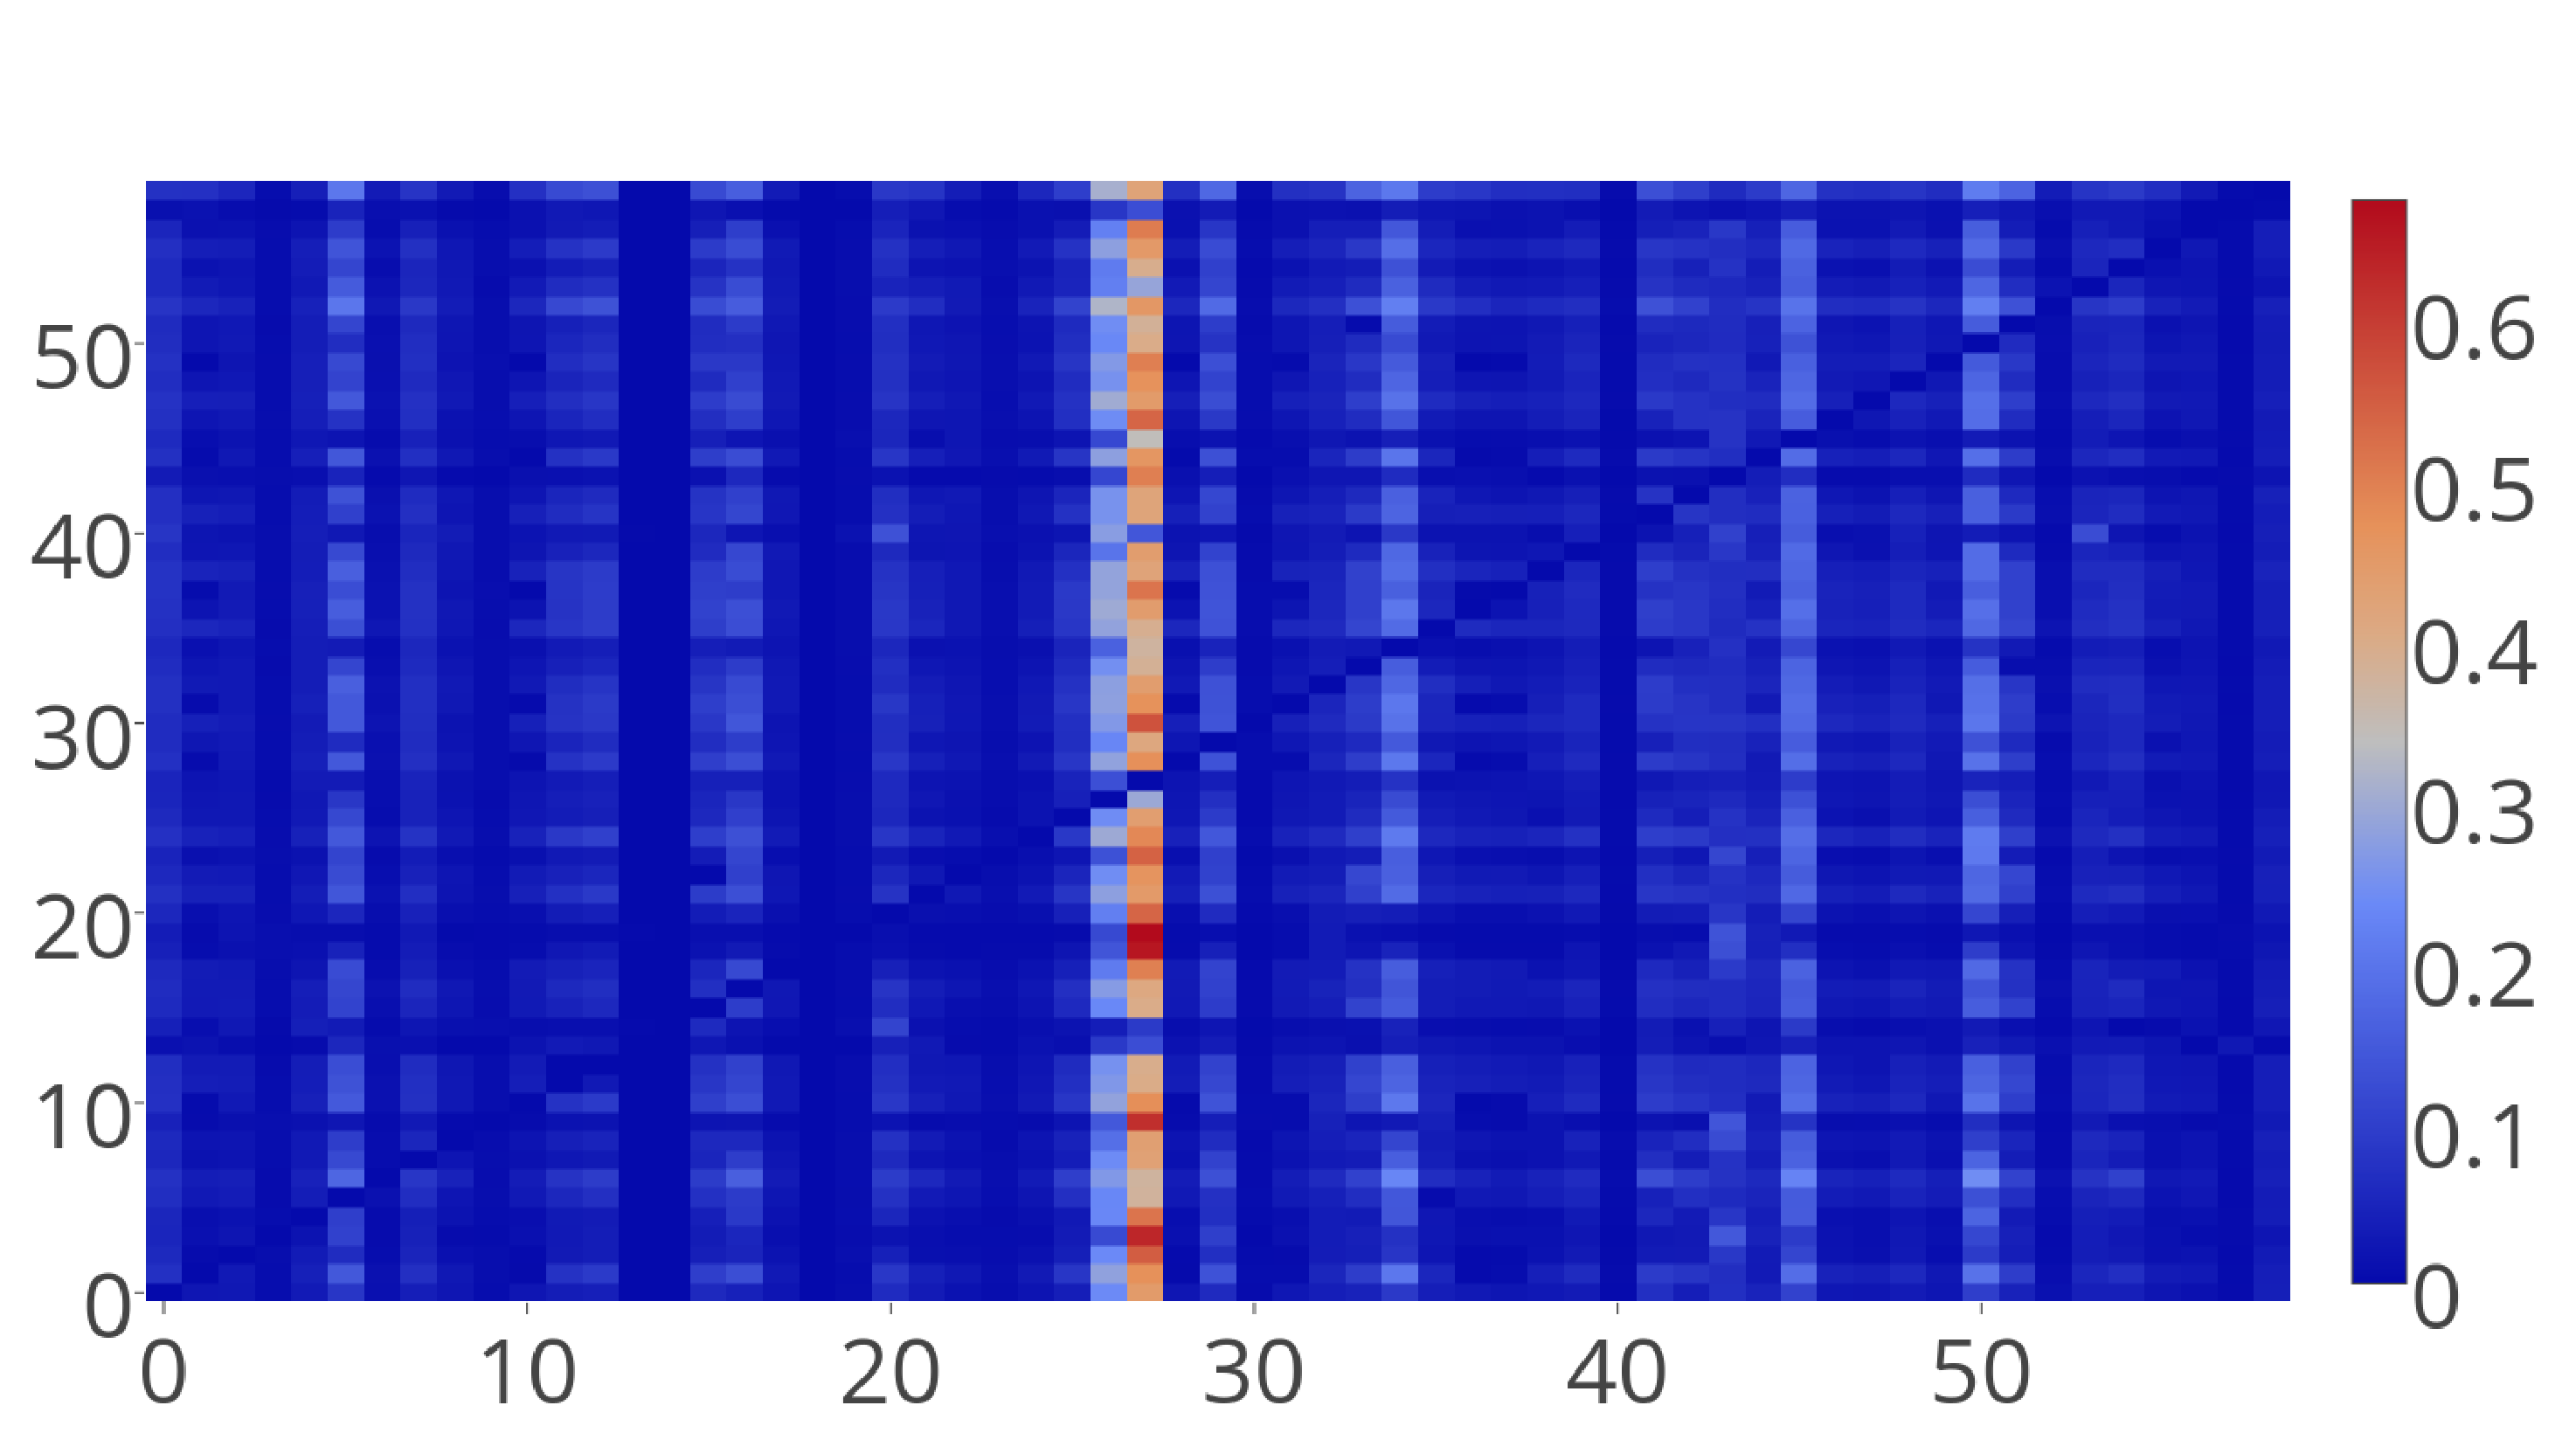
\includegraphics[width=0.24\linewidth]{figure/bernoulli-train}\label{fig:moredata1}} 
\subfloat[]{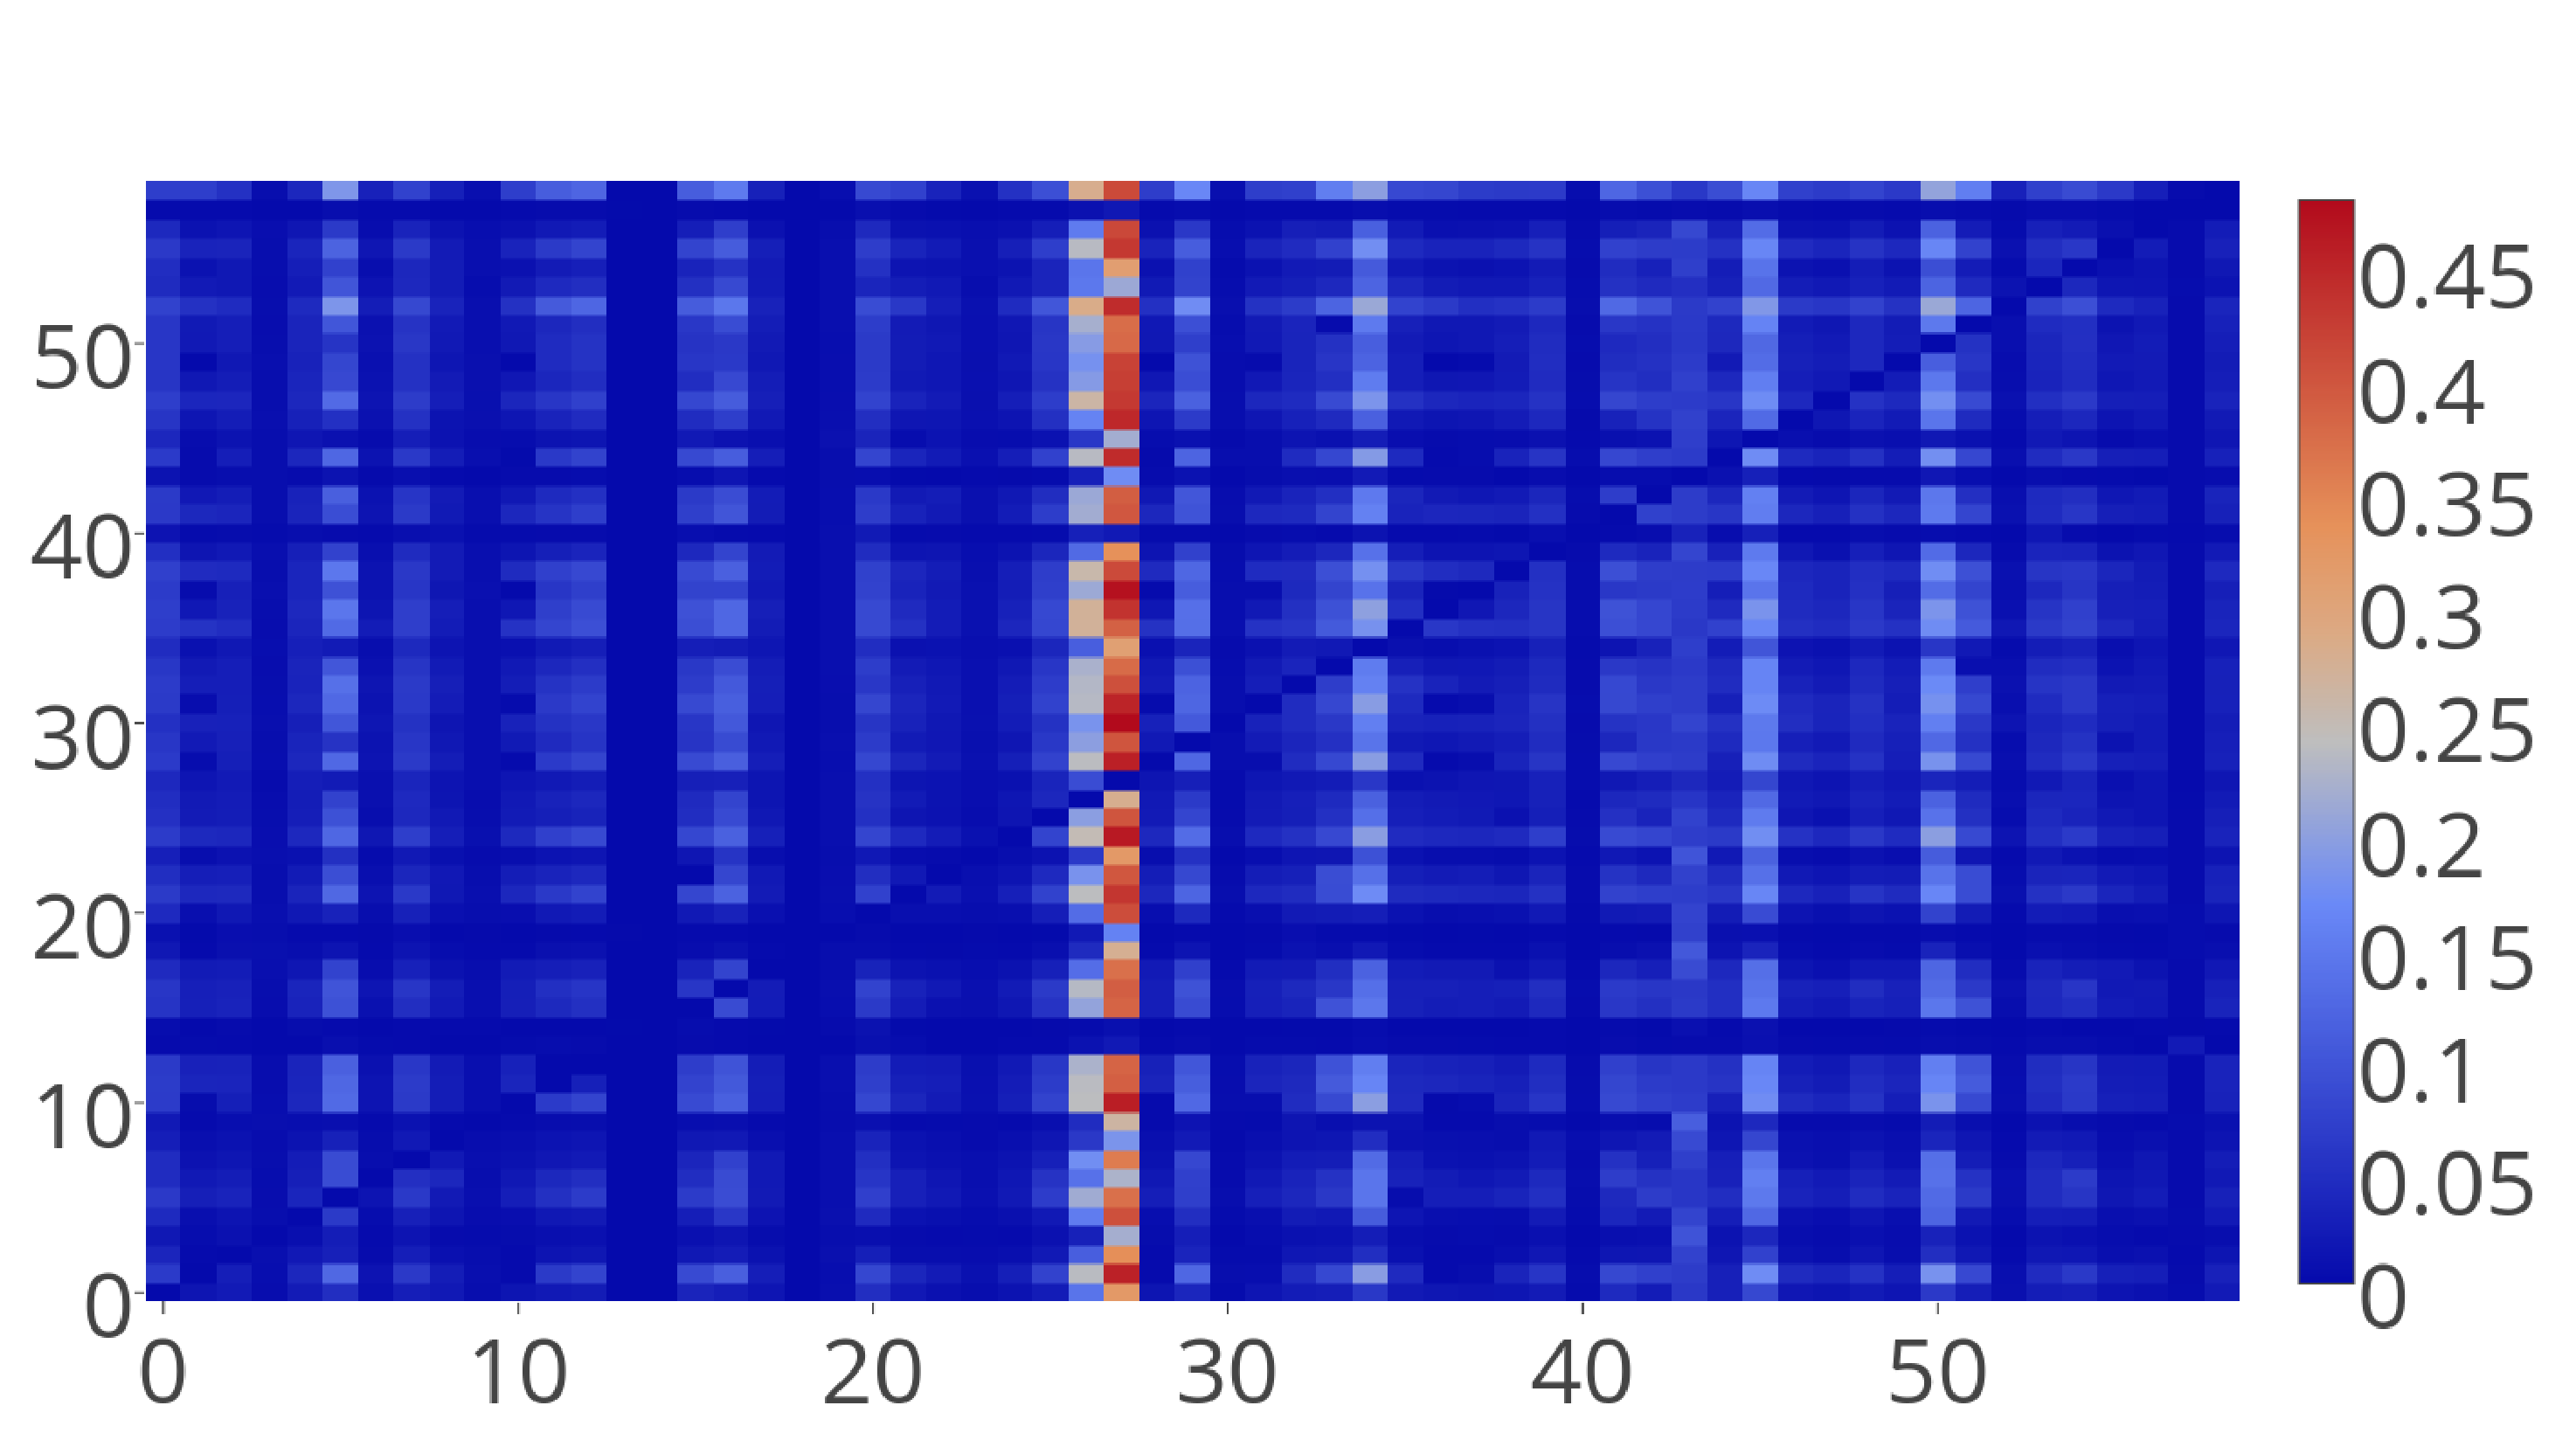
\includegraphics[width=0.24\linewidth]{figure/jaccard-train}\label{fig:moredata2}}
\subfloat[]{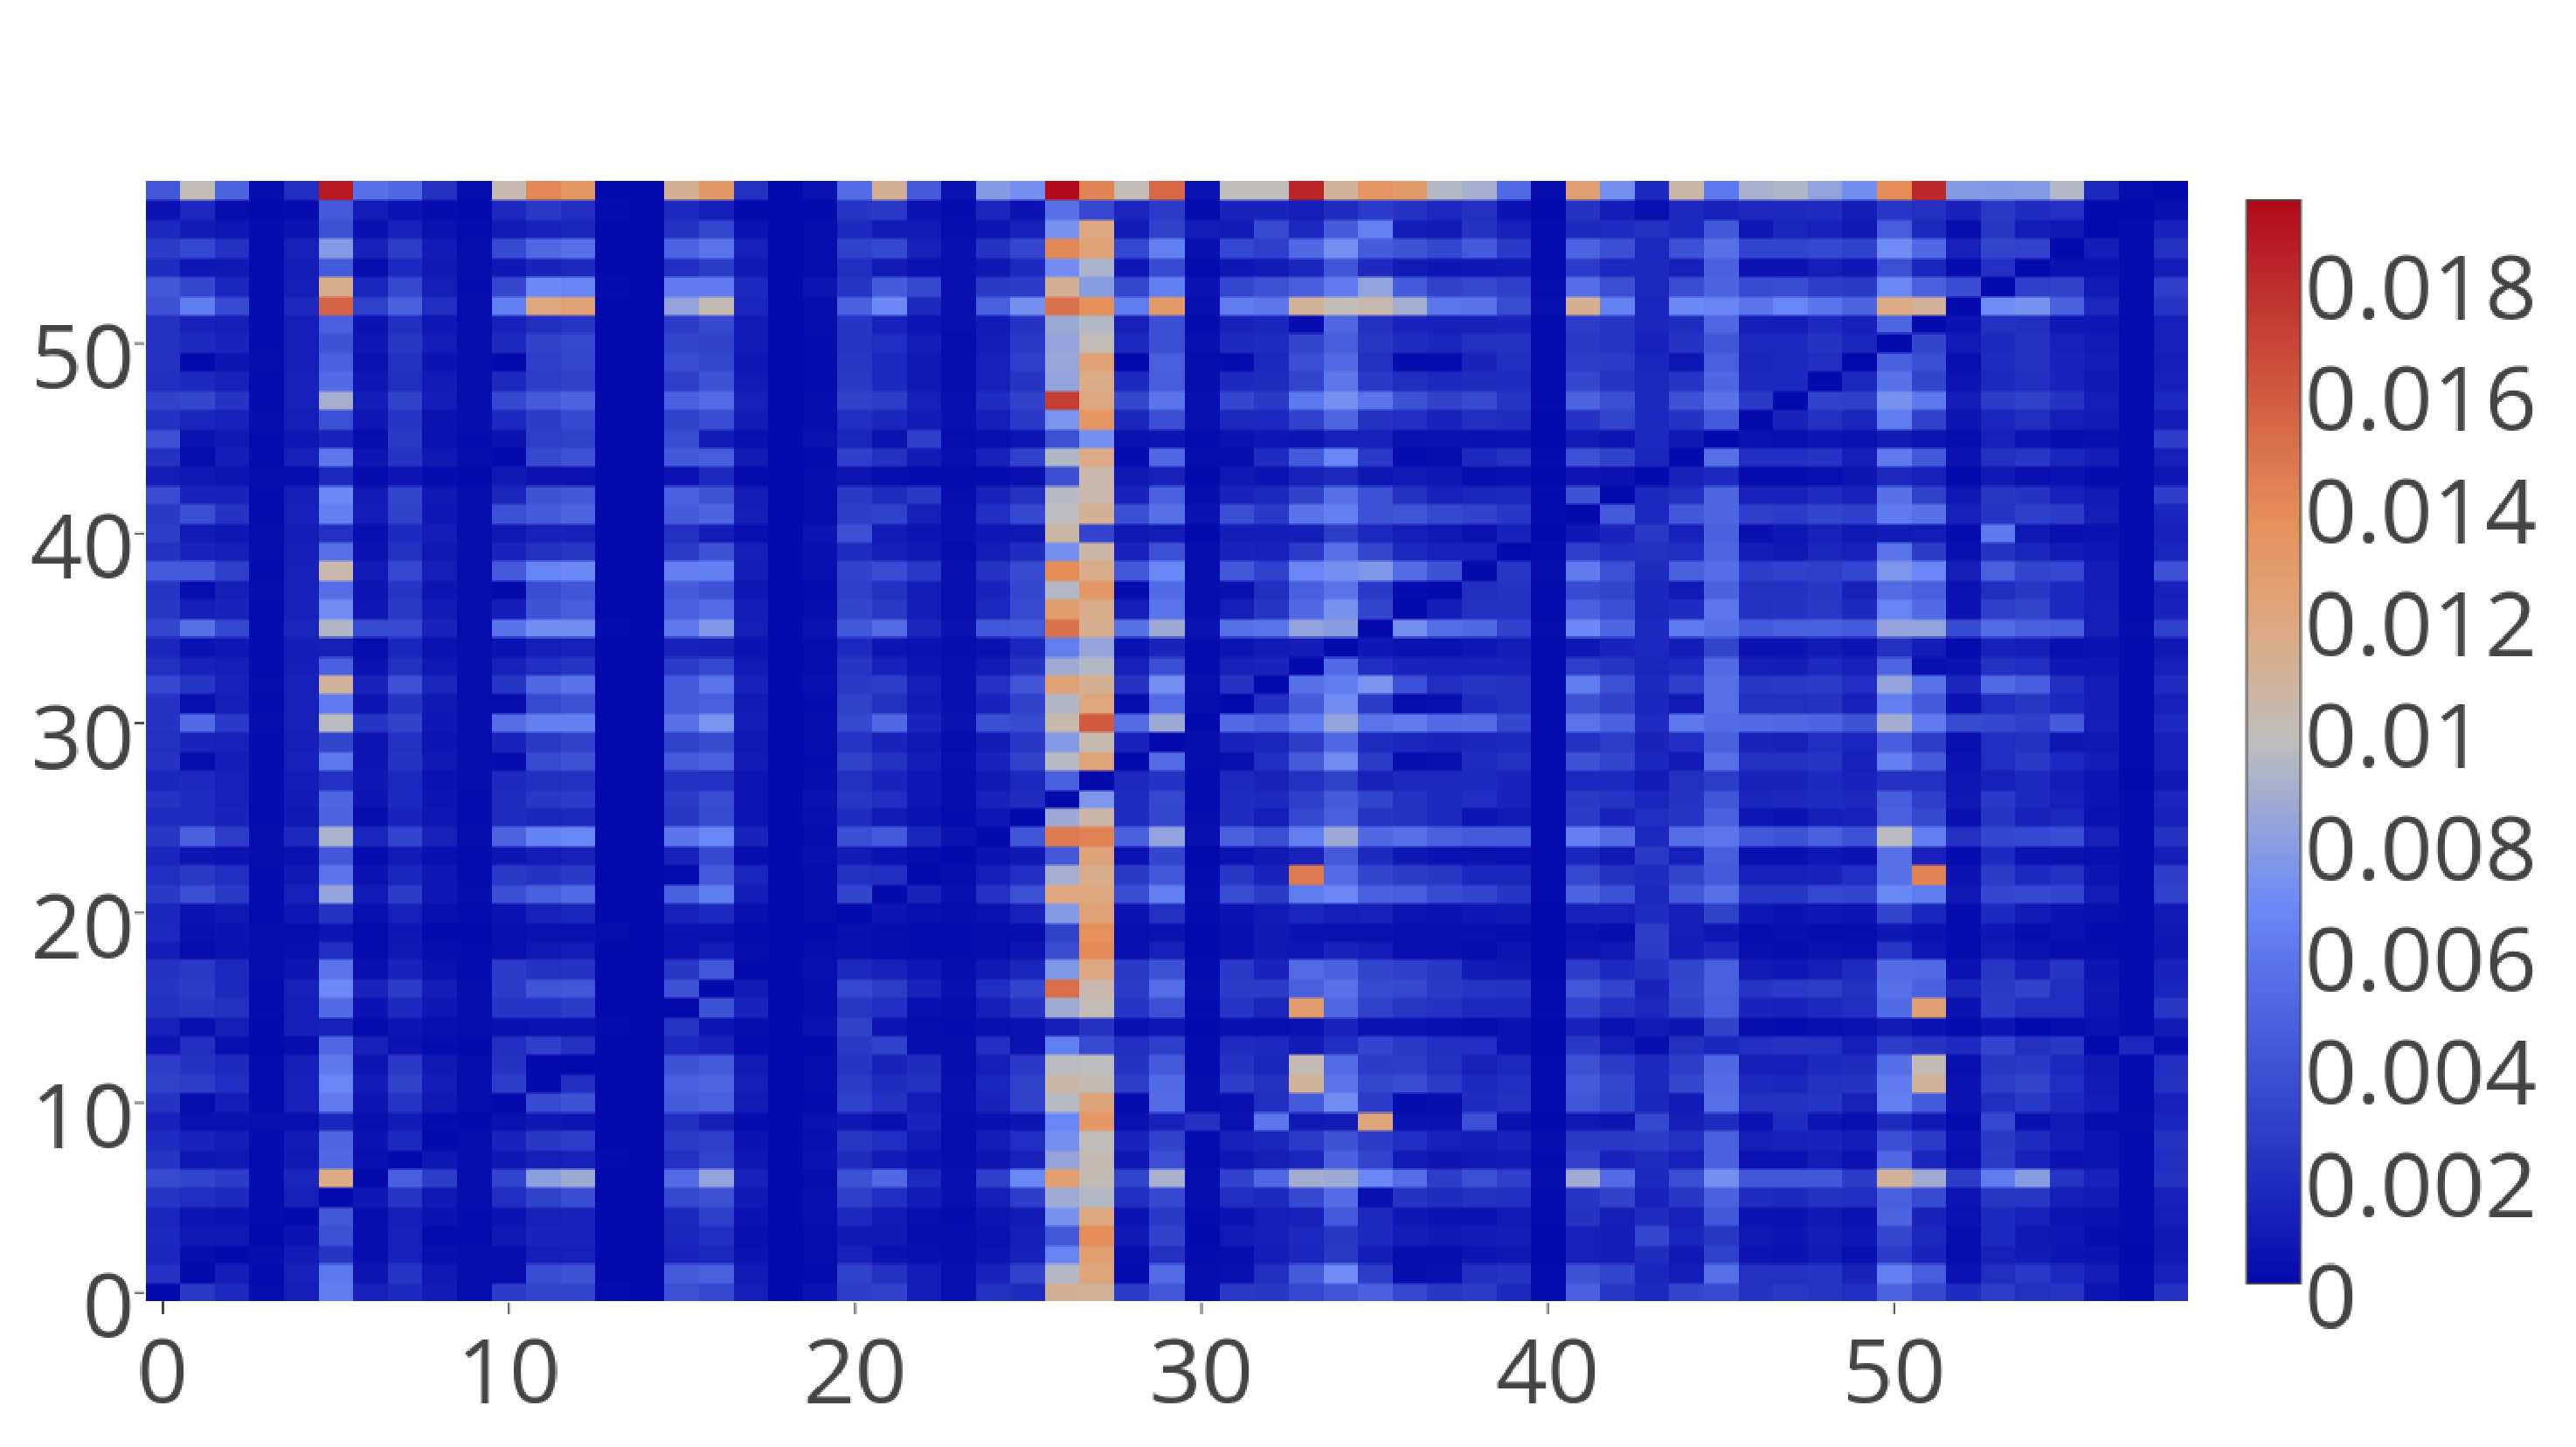
\includegraphics[width=0.24\linewidth]{figure/PC-train}\label{fig:moredata3}} 
\subfloat[]{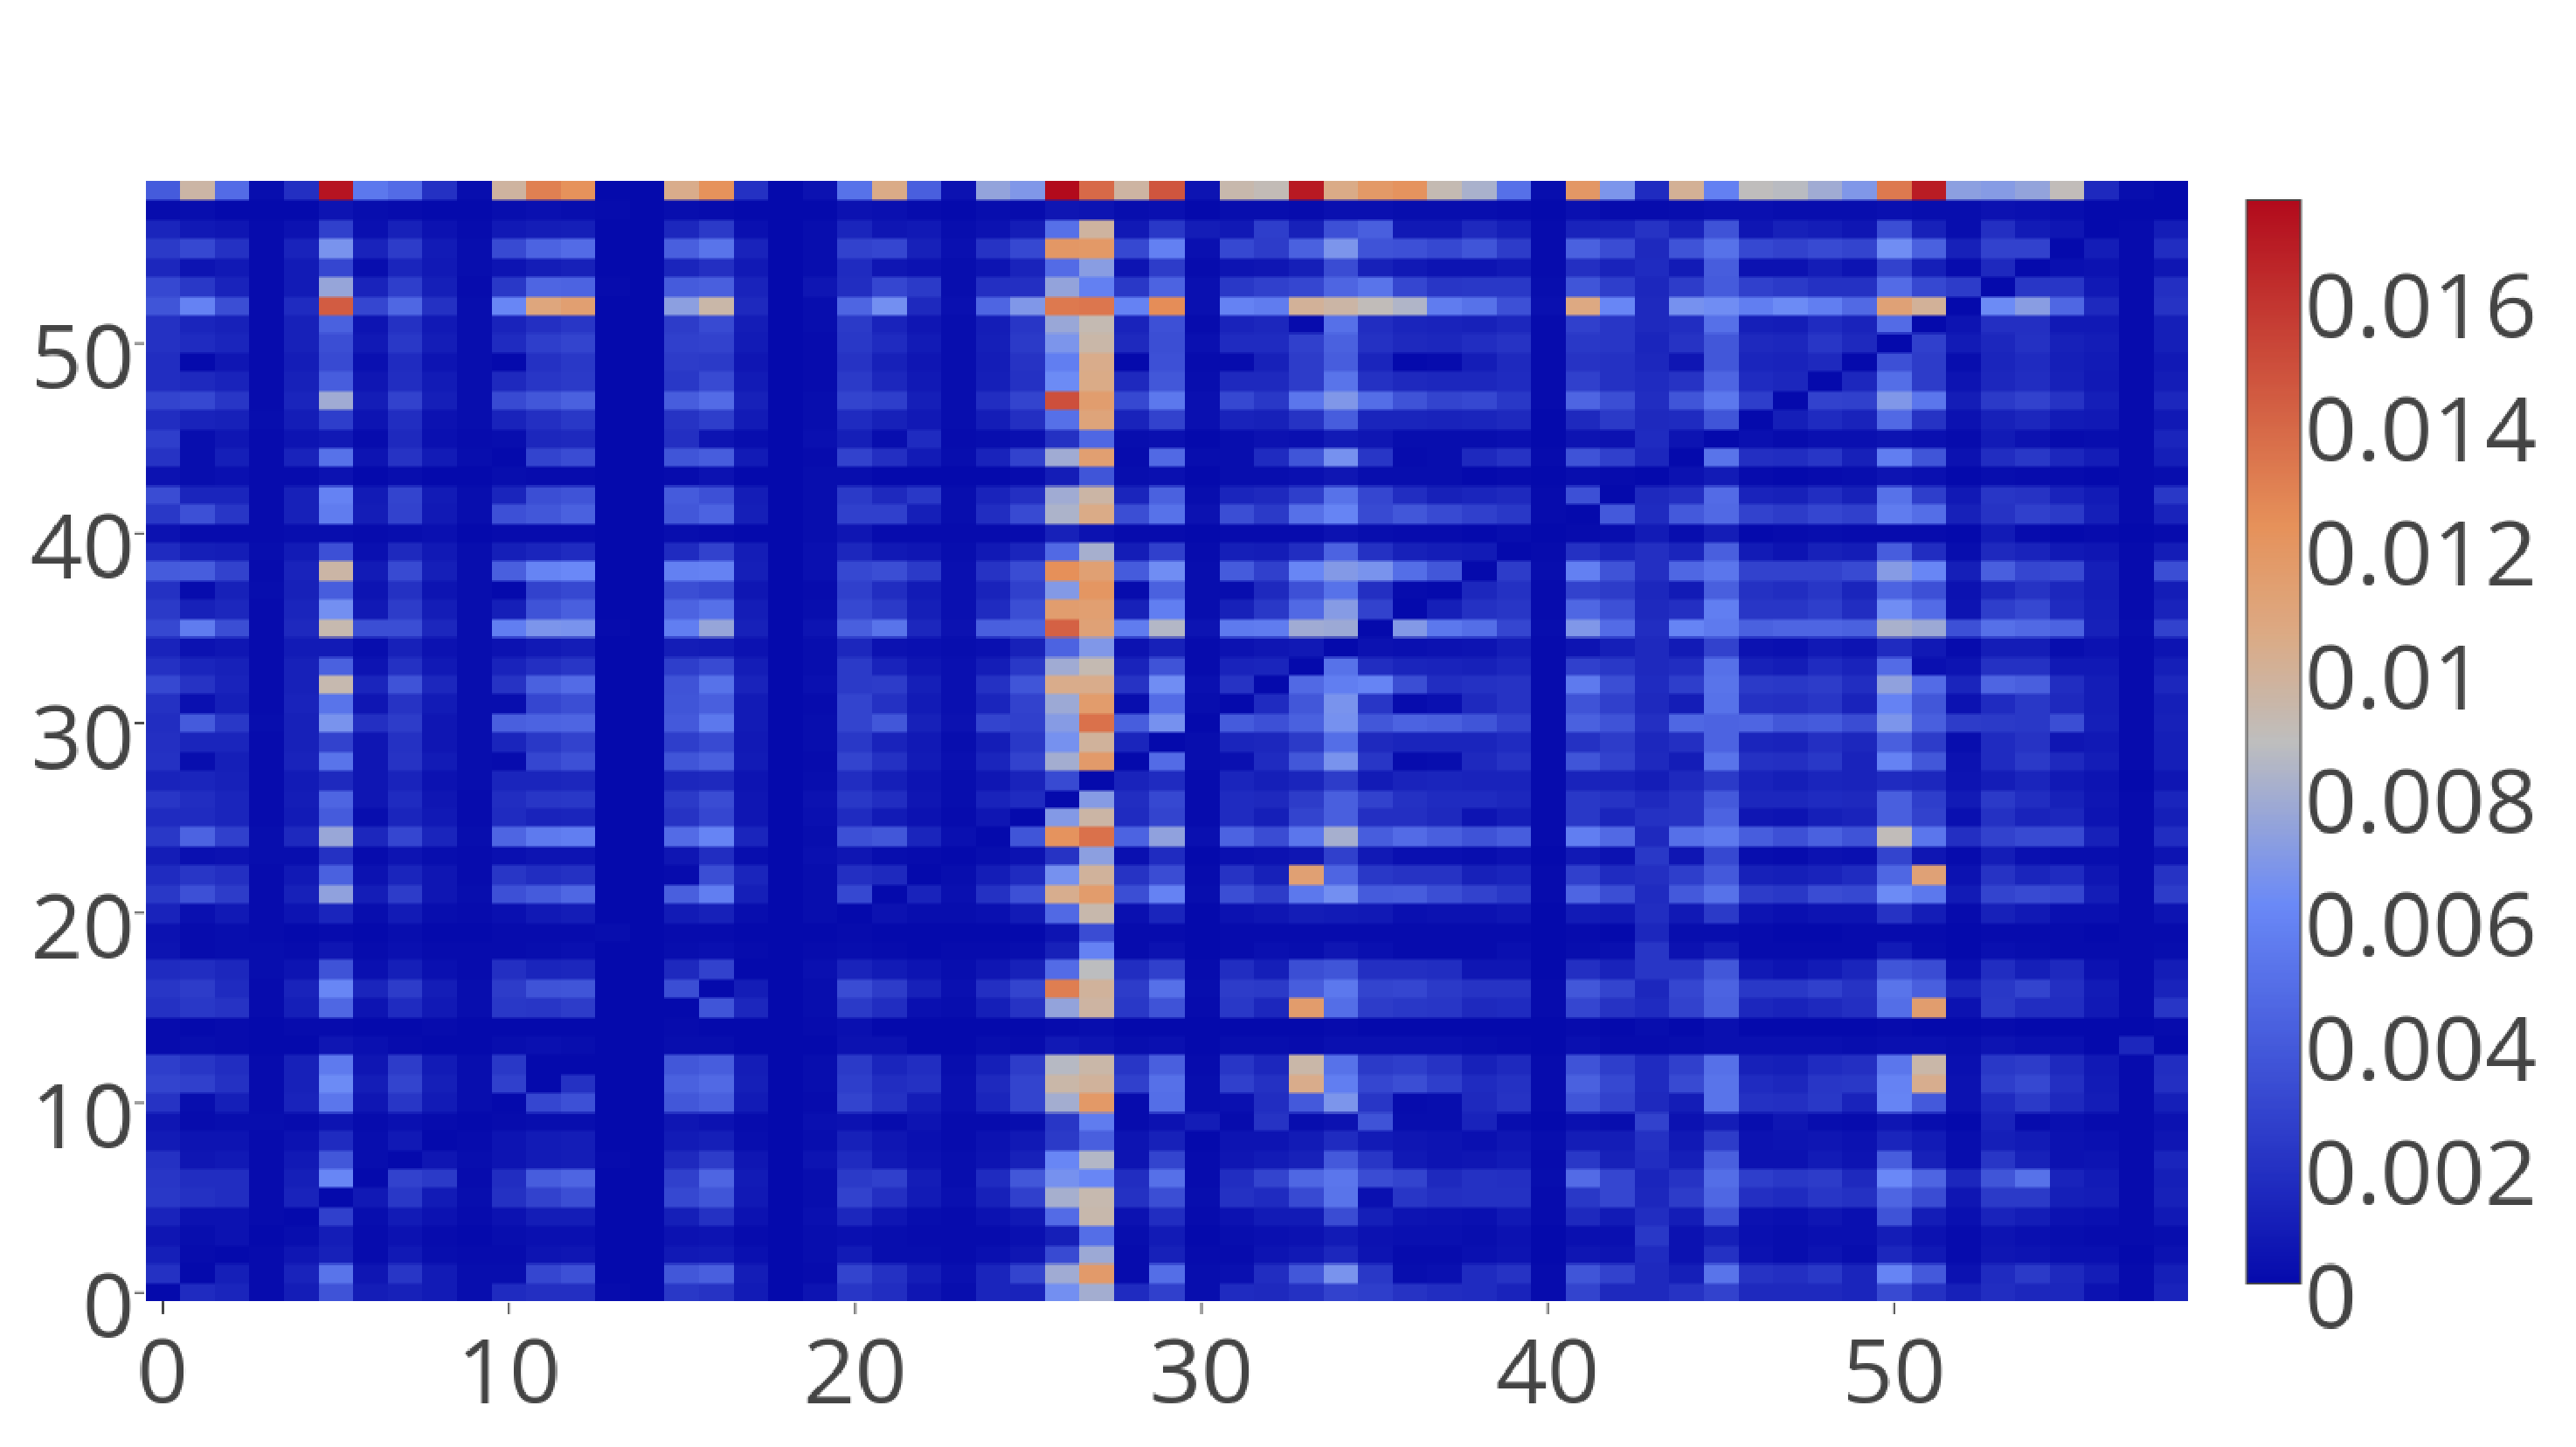
\includegraphics[width=0.24\linewidth]{figure/jaccardPC-train}\label{fig:moredata4}} \\ 
\caption{Potential for 0.5 V bias.} 
\label{fig:EcUND} 
\end{figure*} 


\begin{figure}[t!]
\begin{center}
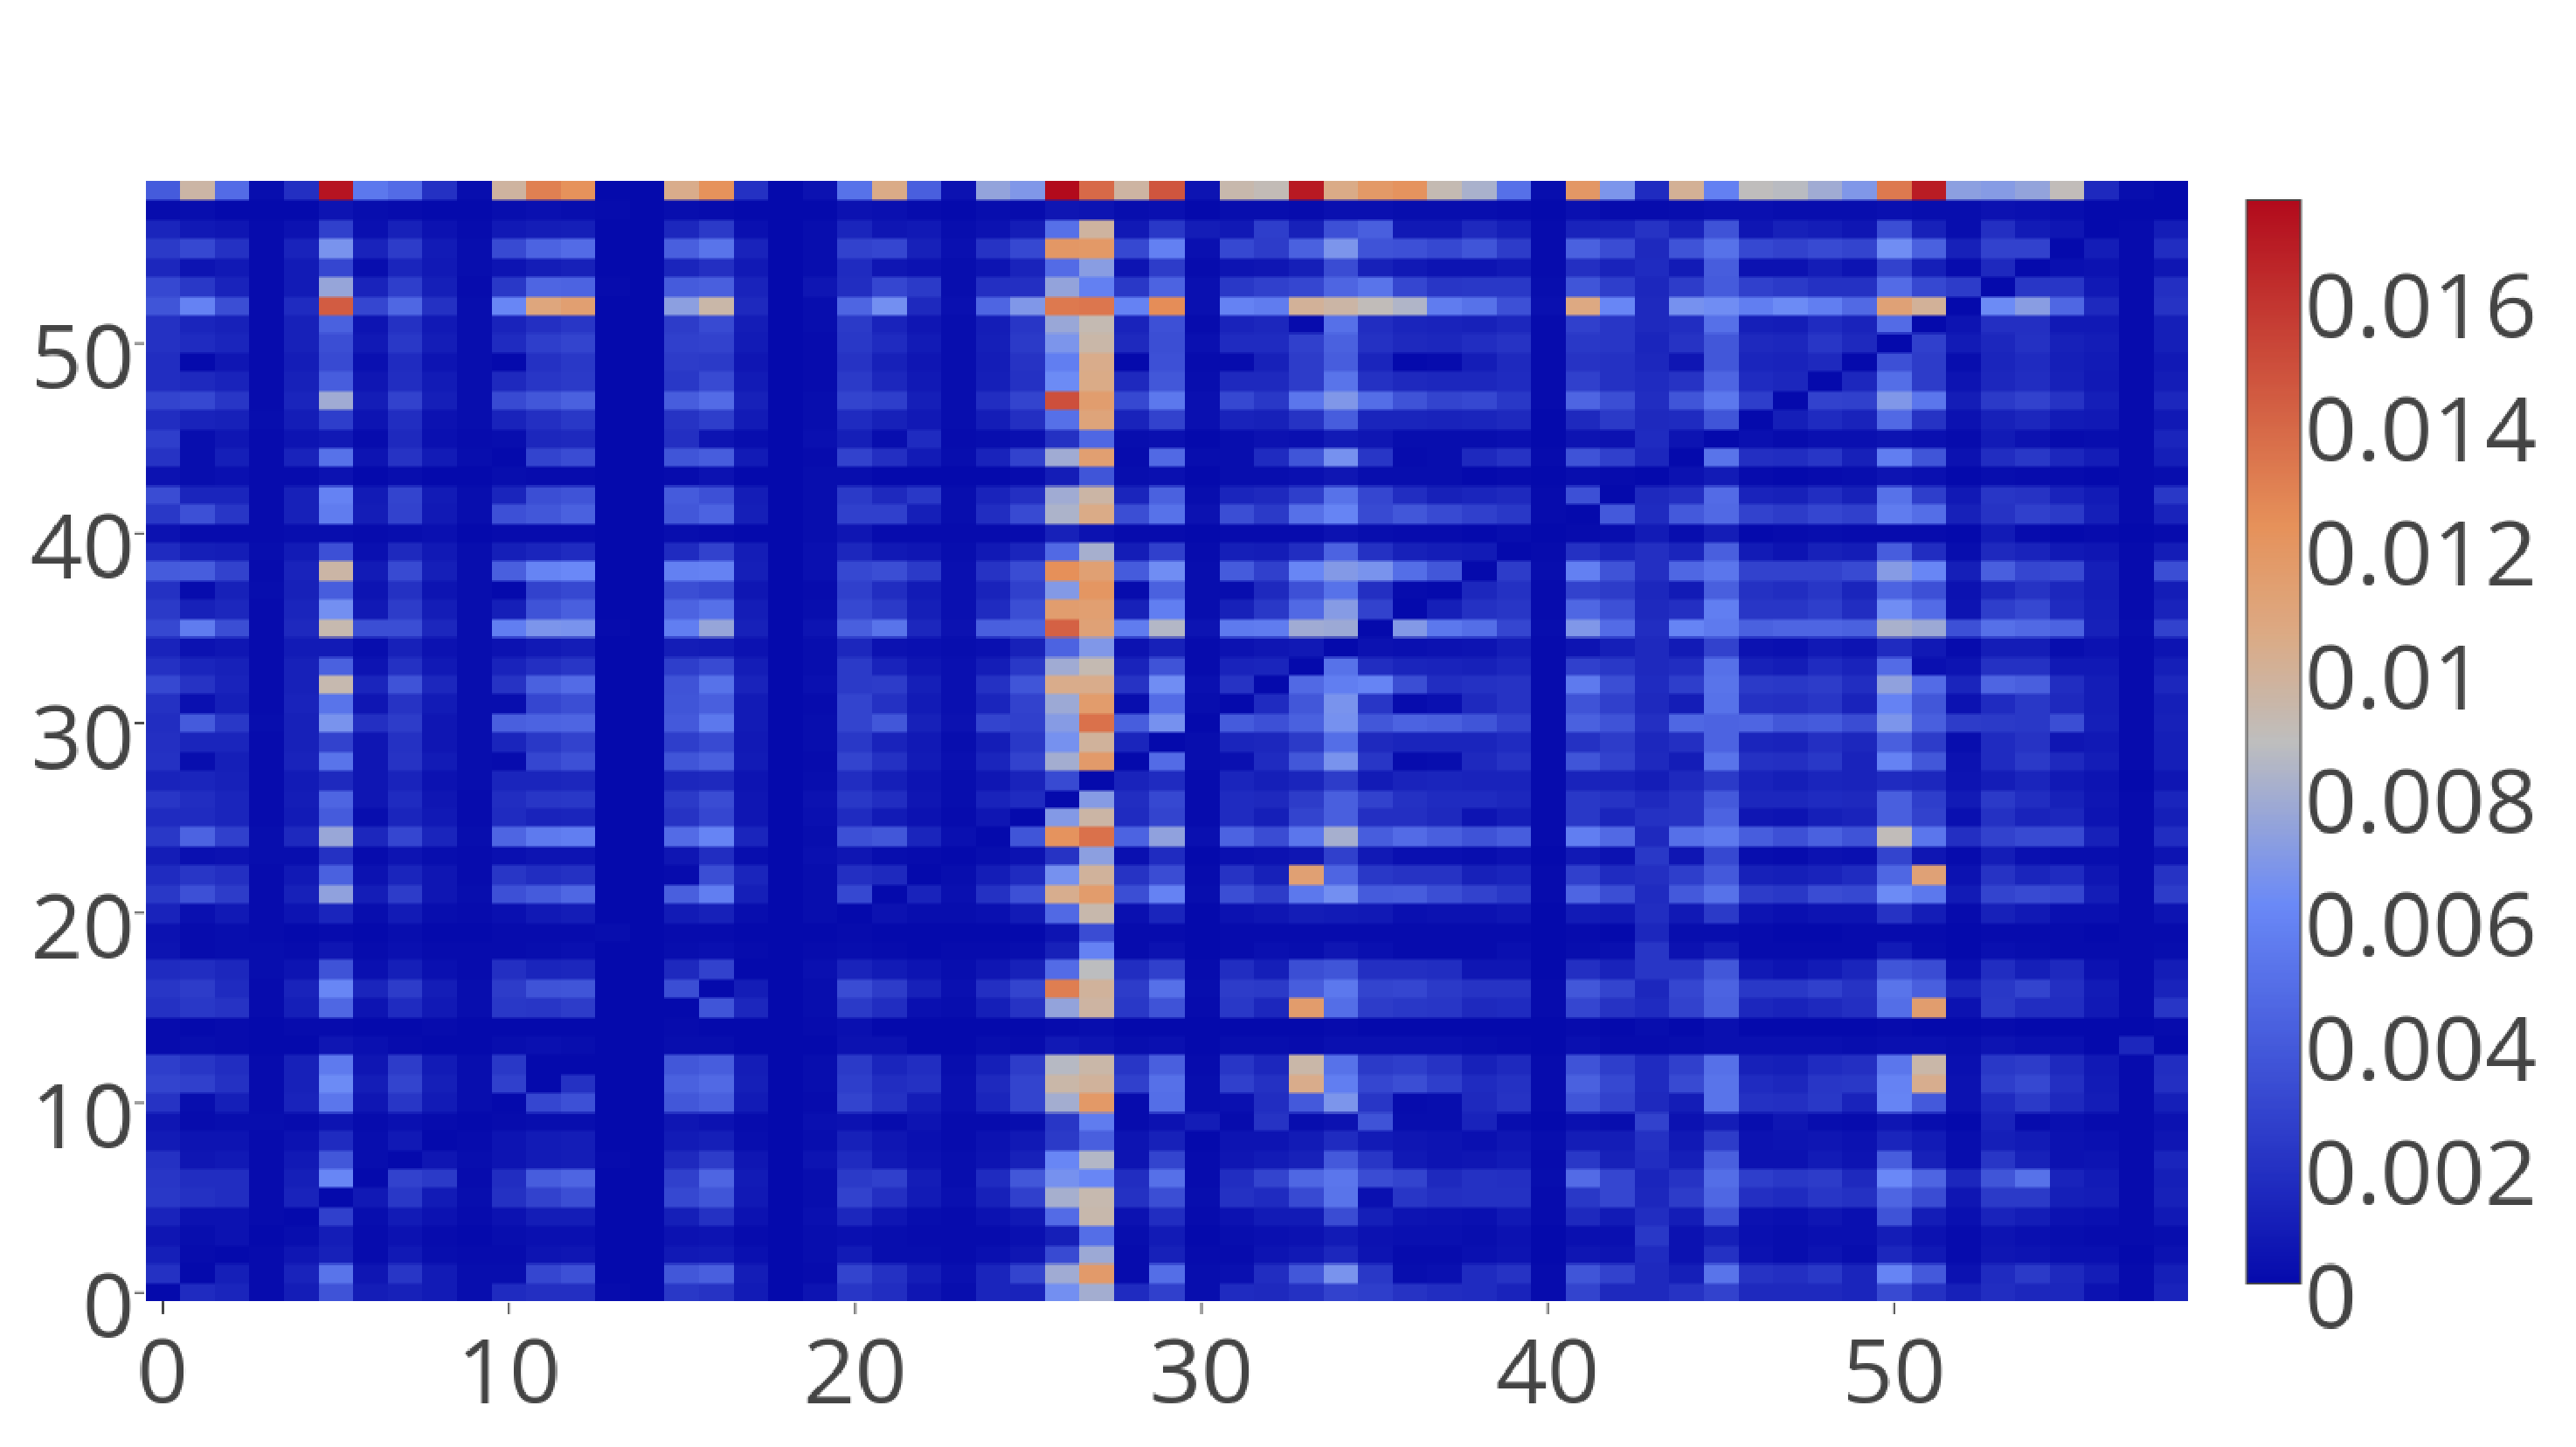
\includegraphics[width=2.5in]{figure/jaccardPC-train}
\mycaption{fig:idreputation}{Test.}
{\footnotesize{(How detection rate changes with the value of source id's reputation. Each reputation is rounded up to nearest 0.05.
Reputation -1 means the source id did not make any submission before. 95\% confidence interval is also drawn 
for each point.)}}
\end{center}
%\vspace{-0.25in}
\end{figure}


\subsection{Influence Probability Analysis}
\label{sec:influenceanalysis}

Using the four static models discussed above, we built an influence graph with anti-virus engines on \vt\ and analyzed 
the influence probability ($p_{u,v}$) between each pair of engines.

\noindent{\underline{\textit{Methodology.}}}
We implement our analysis using several stages of map, filter, and reduce in Spark~\cite{spark}. 
Specifically, we first map submission records according to their corresponding files
and filter out submissions without action propagation. 

\if 0
{\color{red} XXX I don't get the following paragraph. Do we really need this much impl details?}
We then sort submission records for each remaining submitted file chronologically in a map stage.
In the next map stage, we compute four hash tables for each submitted file based on all its submissions.   
There is one one-dimension hash table, containing whether the action to identify the submitted file as malware is taken by each vendor ($|A_{u}|$). 
There are three two-dimension hash tables, 
containing an entry for each pair of vendors $(u,v)$, 
representing whether both $u$ and $v$ take the action ($|A_{u\&v}|$),  
whether the action is propagated from $u$ to $v$ ($|A_{u2v}|$),
and partial credit taken by $u$ if the action is propagated from $u$ to $v$ ($credit_{u,v}(a)$).
After this stage, $|A_{u}|$, $|A_{u\&v}|$, and $|A_{u2v}|$ are either 0 or 1,
and $credit_{u,v}(a)$ is 0 or not larger than 1, since all these values are calculated for one single submitted file. 
In the final stage, 
we reduce these 4 hash tables from different files,
and calculate $p_{u,v}$ for the four static models. 
\fi

We then filter out engines taking fewer than 20000 actions,
since engines taking too few actions cannot produce meaningful results.
There are 59 engines left,
and the average number of actions taken by these engines is around 392K. %190140, which is much larger than 10000.
For confidentiality reasons, we omit vendors' name in the following discussion
and use numbers from 0 to 58 to represent these vendors.

\noindent{\underline{\textit{Analysis results and implications.}}}
For each static model, 
we construct an influence table with calculated influence probability values ($p_{u,v}$), 
with $u$ as row number and $v$ as column number.
We visualize these influence tables with heat maps in Figure~\ref{fig:heat}. 
Each $cell(u, v)$ represents the relative heat color of $p_{u,v}$, 
and red means more influence from $u$ to $v$. 

We also sum all $p_{u,v}$ values in a column in each influence table 
to calculate trustworthiness of engine $v$ using Equation~\ref{eq:trust}. 
Table~\ref{tab:trust} lists the maximum, minimum, and average trustworthiness values of all the engines under four different models.
The results can serve as a quantitative measurement for how trustworthy anti-virus engines are. 

In all the four heat maps, there are two columns with almost all cells in red,
which means that these vendors influenced by all other vendors and are less trustworthy.
On the other hand, quite a few vendors are not influenced by any vendors (blue columns).
This result suggests that most vendors perform predictions on their own and thus can be trusted. 
However, our result should also ring an alarm to online malware detection service users and security experts that 
we cannot treat all engines with the same level of trust 
and the results from some of them should be at least examined more closely if not discarded.

At the same time, there are several rows with many cells in red, especially in the last two heat map, 
which means that there are vendors which influence many vendors,
where there are a set of vendors that do not influence other vendors (blue rows).
Different from the effect of columns which shows the trustworthiness of a vendor by users, 
the effect of rows is related to how vendors view (and trust) each other. 
Certain vendors are highly regarded by many other vendors so that 
their decision results are often referenced by other vendors.

Interestingly, the vendors that are heavily influenced by others are not the ones that influence others, 
suggesting that the vendors with lower trustworthiness by users are also not trusted by other vendors. 

\begin{table}[h!]
\centering
\footnotesize
{
\begin{tabular}{l|l|l|l}
\hline
Model                & Max     & Min & Average \\
\hline                            
%\cline{1-1}
{\bf Bernoulli}                    & 108.78   & 0.04 & 5.40 \\
{\bf Jaccard Index}                & 118.20   & 0.05 & 6.15 \\
{\bf Bernoulli with Partial Credit} & 3545.34  & 1.63 & 138.45 \\
{\bf Jaccard Index with Partial Credit} & 4177.98 & 2.02 & 155.18 \\
\hline
\end{tabular}
}
\caption{Trustworthiness. 
%\footnotesize{
(Maximum, minimum, and average trustworthiness values under four different models.)
%}
}
\label{tab:trust}
\end{table}


Finally, we observe that although the four static models show similar trends of influence relationship 
and the relative rankings of engines in terms of influence are similar,
their absolute influence probability values differ. 
Bernoulli distribution and Jaccard index have influence probability values
that are about 30 to 40 times higher than
Bernoulli and Jaccard index with partial credit. 
%This shows that {\color{red} influence is shared among vendors take actions earlier than others. I have no idea what sentense means. if you cannot explain well, just remove this sentence.}.

{\bf Observation 8:} 
{\em Certain anti-virus vendors are influenced by almost all other vendors in their malware detection decisions and are less trustworthy, 
while quite a few trustworthy vendors have influence on many other vendors.}

\subsection{Influence Probability Prediction}
\label{sec:predict}

The analysis results of vendor influence above are encouraging.
With these results, we take a step further and ask 
{\em if it is possible to predict whether or not an engine's prediction of 
a file submission should be trusted (i.e., not influenced by other engines)?}
We now discuss the prediction model we built to answer this question.

\noindent{\underline{\textit{Methodology.}}}
We first split all the \pe\ submissions we collected into a training set and a testing set based on 
the SHA256 values of the submitted files. 
We place all submissions with SHA256 values starting with a numeric character, 
i.e., from `0' to `9', into training set
and all the rest (starting from 'a' to 'f') into the testing set.
We use Spark to implement both the training and the testing process.
%Similar to our training stage process, 
%we first reduce all submissions based on submitted files,
%next filter out files without action propagation, 
%and then sort submissions chronologically. 


%\noindent{\underline{\textit{Training stage methodology.}}}
During the training stage, we use the training set to build an influence graph and
learn $p_{u,v}$ of each edge in the graph using the four static models discussed in Section~\ref{sec:influenceprob}.
The calculation of $p_{u,v}$ is the same as in Section~\ref{sec:influenceanalysis}.

%\noindent{\underline{\textit{Testing stage methodology.}}}
During the prediction stage, for each submission in the testing set, 
we predict whether or not an engine $v$ will take an action $a$ following other engines 
if it has not taken that action yet. 
%Specifically, we use a tunable threshold $\theta$
%and predict $v$ will follow its neighbors to take the action $a$ in the future
%if $p_v(S_v(a))>\theta$.
Specifically, to test a submission, we first use Equation~\ref{eq:setp} to
calculate $p_v(S_v(a))$, the probability that $v$ will follow its neighbors to take the same action, 
for all engines that have labeled the submitted file only as benign in their history. 
These engines are of interest to us because positive influence, 
the type of influence in this study, only happens 
when an engine changes its prediction decision from benign to malware.

We then compare $p_v(S_v(a))$ with a {\em tunable threshold $\theta$} to predict whether $v$ will label the file as malware (if $p_v(S_v(a))>\theta$) or not.
Next, we compare this prediction with the actual action that $v$ took in the testing set to deduct true positives (TPs) where both our prediction 
and the actual fact label the submission as malware, 
false negatives (FNs) where our prediction labels the submission as benign and the actual labeling is malware. 
Thus, TP means our prediction is the same as the fact 
and both show the engine changes its labeling from benign to malware, an indication that the decision 
of this engine on the submission is in deed affected by other engines.
Similarly, we can obtain false positives (FPs) 
and true negatives (TNs).
%After processing all submissions for a file, 
%we calculate $p_v(S_v(a))$ for all engines  
%that label the file as benign but have not labeled the file as malware.
%We compare $p_v(S_v(a))$ with $\theta$ to count false positives (FPs) and true negatives (TNs).
In the final stage, we calculate the overall TP, TN, FP, and FN rates for all different files.

\begin{figure}[t!]
\begin{center}
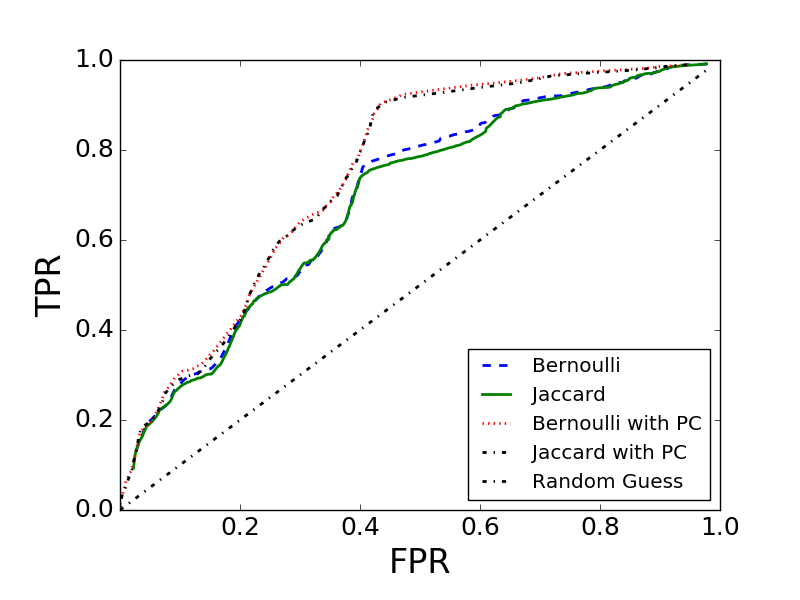
\includegraphics[width=2in]{figure/predict}
\vspace{-0.1in}
\caption{ROC comparisons of Static Models. 
(How true positive rate (TPR) changes with false positive rate (FPR). 
We change probability threshold from 0.1\% to 99.9\% with step 0.1\%. 
We compute TPR and FPR for each probability threshold to draw the curve.)
}
\label{fig:predict}
\end{center}
\vspace{-0.1in}
\end{figure}

\noindent{\underline{\textit{Prediction results.}}}
We change the threshold $\theta$ from 0.1\% to 99.9\% 
and measure the accuracy of the four static models using ROC (Receiver Operating Characteristic) curves,
with true positive rate ($TPR = TP/(TP+FN)$) as X-axis
and false positive rate ($FPR = FP/(FP + FN)$) as Y-axis. 
Figure~\ref{fig:predict} plots the ROC curves for the four static models.
A larger area under the ROC curve means higher accuracy.
We compare our prediction models with random guess, 
which is represented by the diagonal line between (0,0) to (1,1) in the figure. 

We find that all models are more accurate than random guess
and using partial credits improves the accuracy of both Bernoulli and Jaccard index.
This result is encouraging;
even with a simple prediction model like ours, we can already obtain satisfactory prediction accuracy of whether an engine's decision has been influenced by others.

{\bf Observation 9:} 
{\em Our influence prediction model can accurately predict whether or not an anti-virus engine's labeling of a submission should be trusted. }

\subsection{Discussion}
%Our scientific analysis on vendor influence in this section confirms our XXX
Our findings in this section shed light on how vendors can influence each other and rings an alert towards using detection rate as the only measurement of the likelihood of a file being malware.
Our study results can serve as a quantitative measurement for vendors' influence in malware detection community. 
Previously, when combining results from different vendors, 
security experts simply treat each vendor equally and use the percentage of 
vendors labeling a file as malware as likelihood of the file to be a malware. 
Our model can provide a weight to each vendor 
when combining results from different vendors.  
Anti-virus vendors can also use our prediction model to detect possible false negatives in their products.

\if 0
{\color{red} Do we really need this (the following two paragraphs)? this sounds very defensive}
%\if 0
There are also time models proposed by~\citet{Influence}.
When analyzing Flickr data, time models leverage accurate action time to provide better prediction performance. 
However, we do not use time models, 
because time information we access is when a submission is conducted, 
or when an engine analyzes a submission, 
is not when an engine changes its detection label for a file.
The time information we have can only provide a relative order about when each vendor identifies a file as malware.  

%\underline{Limitation.}
Our data collection ends on September 6th, 2016. 
We could count extra FPs, where we predict engines will label files as malware, engines have not, but will do in the future, 
and TNs, where we predict engine will not label, engines have not, but will in the future. 
Monitoring \vt for a longer time will make the evaluation of our prediction models more precise. 

%\underline{How to use?}
\fi

